
 En utilisant la formule suivante, on peut calculer la longueur du fil si l'on connait la vitesse de transmission dans notre fil et le temps de transmission:
 
 \begin{equation}
 v = \frac{\Delta X }{\Delta T} \label{eq:equation-vitesse}
 \end{equation}
 
 Donc, en utilisant les résultats suivants obtenus en prenant la mesure entre l'émission de l'onde et sa réception à l'autre extrémité du circuit
 ,comme la figure ci-dessous le démontre, On peut arriver aux résultats suivants.

 \begin{figure}[H]
    \centering
    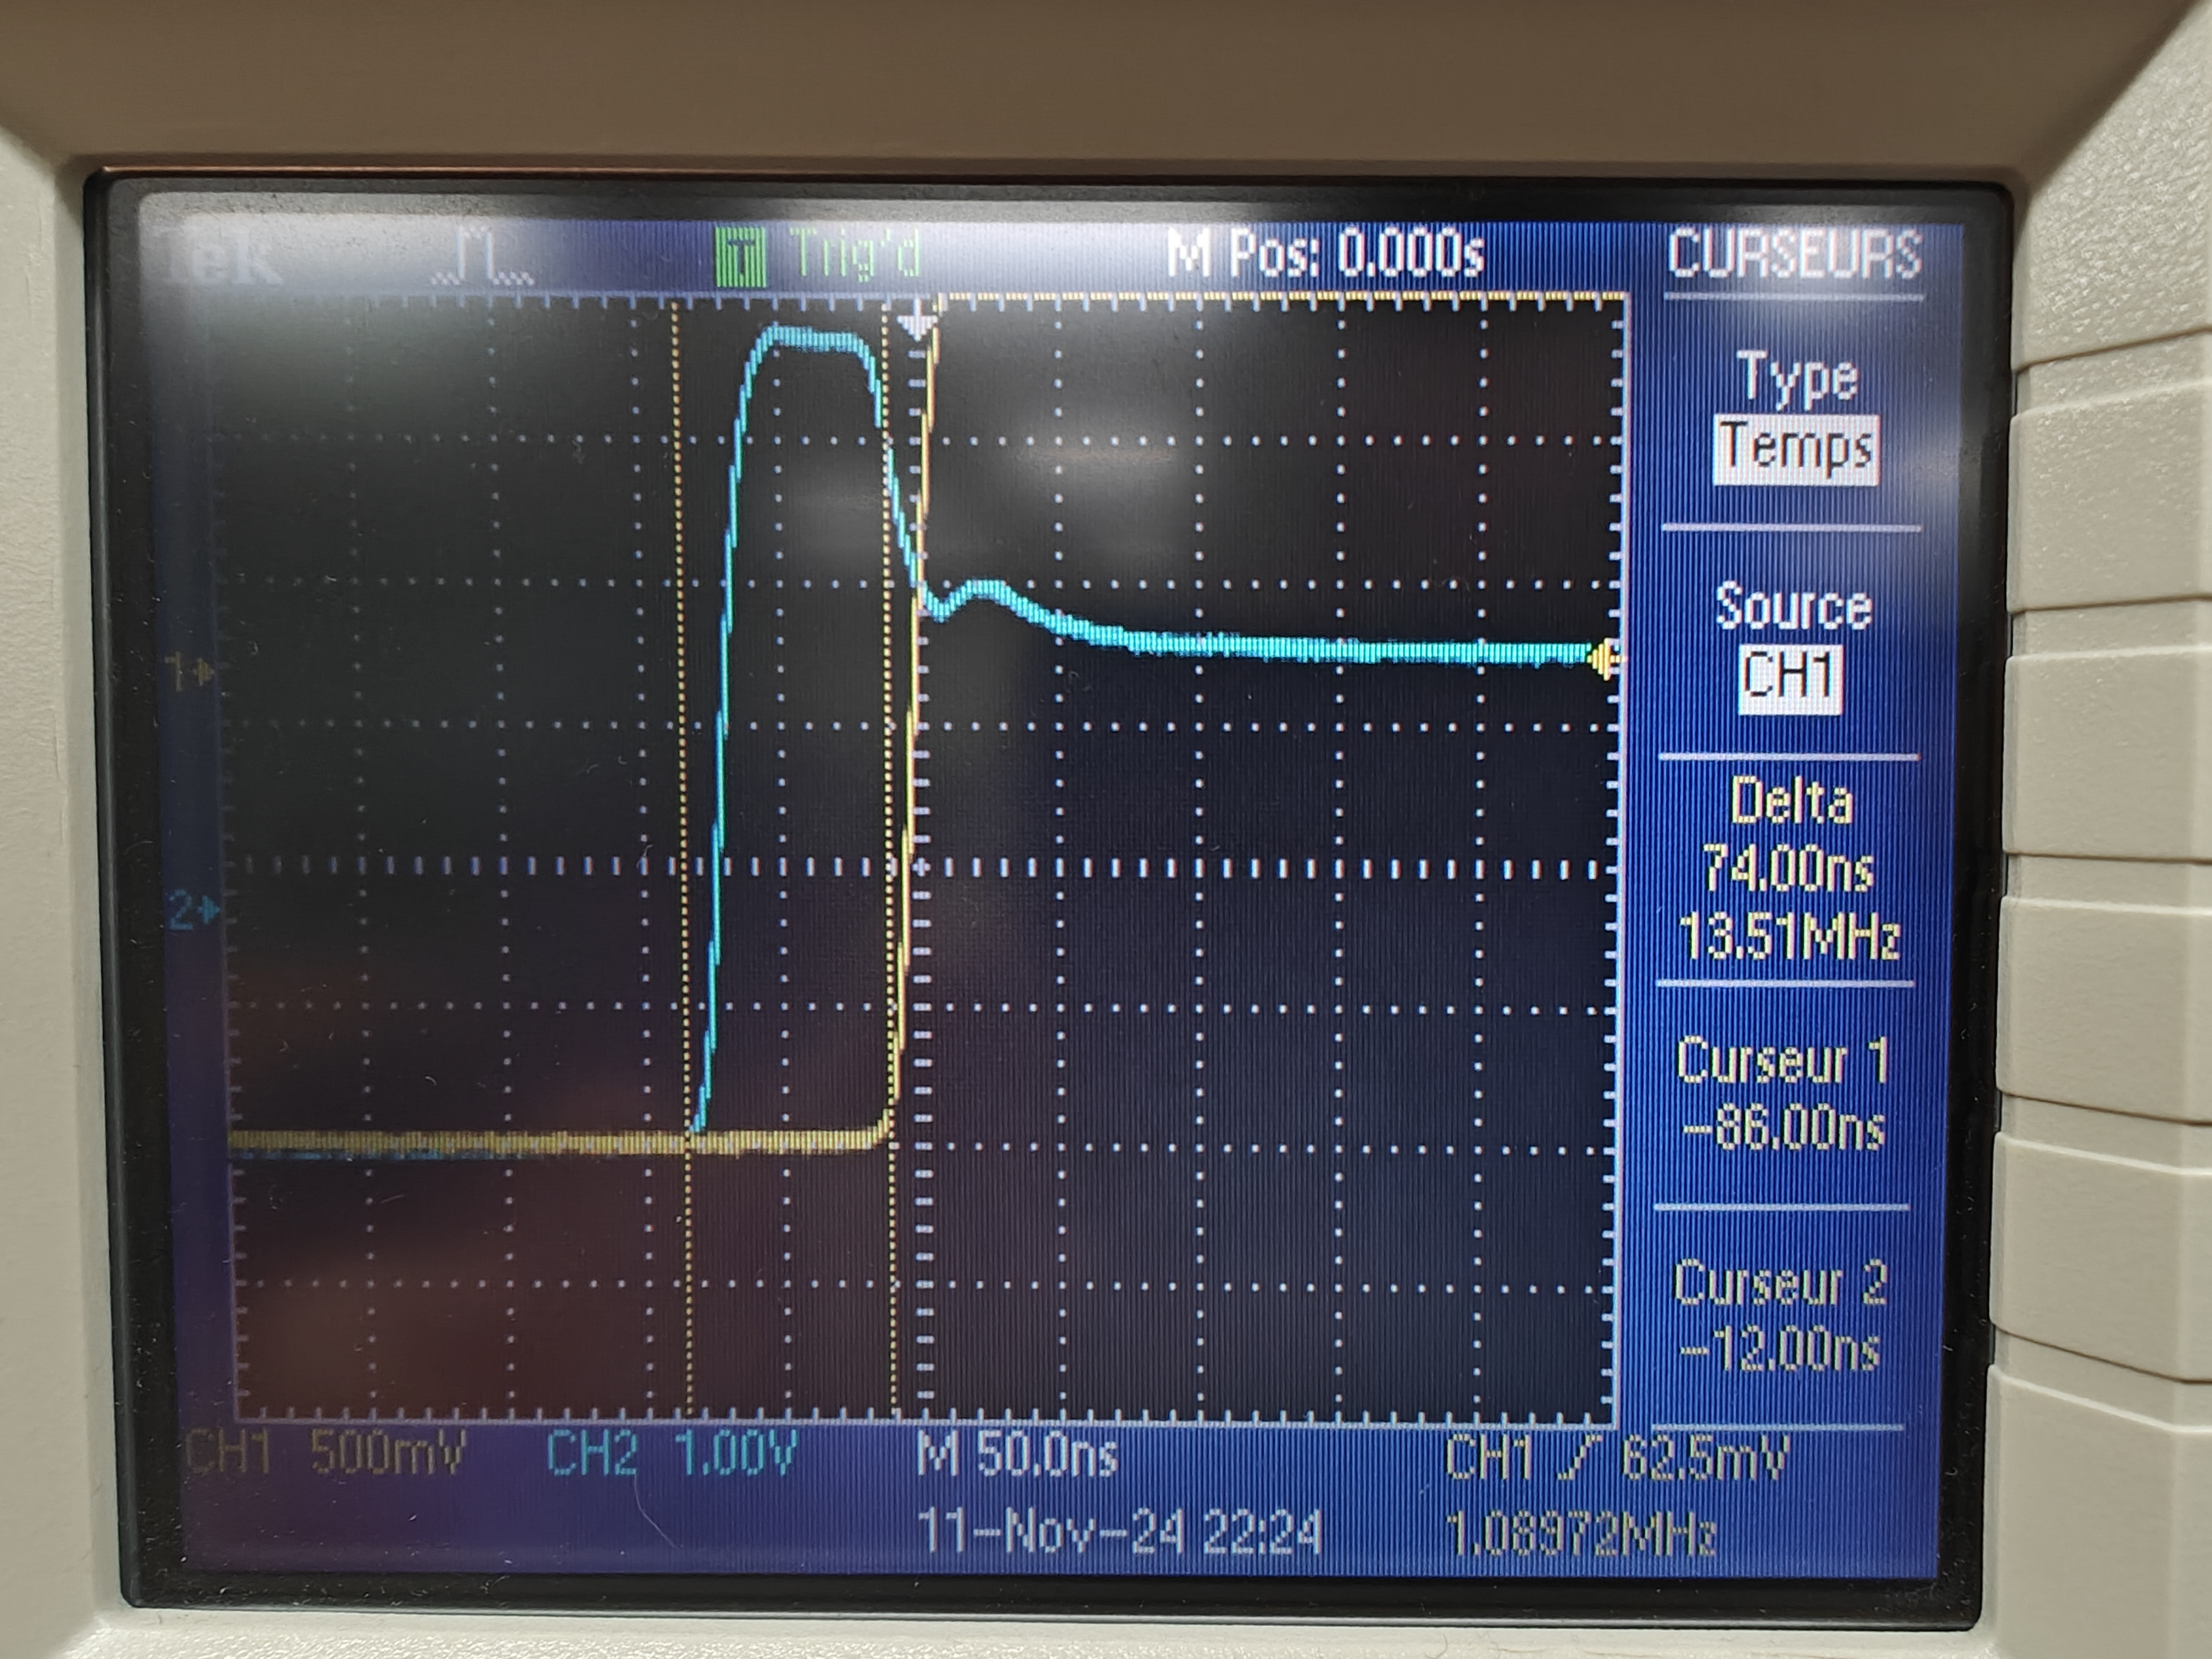
\includegraphics[width=0.7\textwidth]{images/a-b-temporel.jpg}
    \caption{Mesure temporelle du temps de réception du signal}
    \label{fig:analyse-temporelle-a-b}
 \end{figure}


 \begin{center}
 \begin{table}[H]
 \caption{Résultats des mesures temporelles} \label{tab:tableau mesures temporel}
 \begin{tabularx}{\textwidth}{ X X X X }
    Fil d'entrée & Fil d'extrémité & Fil ouvert & Résultat (ns) \\
    \hline
    \hline
     A & B & C & 74\\
     B & C & A & 60\\
     C & A & B & 52\\
     \hline
 \end{tabularx}
 \end{table}
 \end{center}


 La vitesse de transmission assumée du fil est de 2/3 de la vitesse de la lumière, ce qui donne: 
 \begin{equation}
    2*10^8 \frac{m}{s}
    \label{vitesse-transmission}
\end{equation}

 On peut donc obtenir les résultats suivants en utilisant nos mesures et la formule de vitesse \ref{eq:equation-vitesse} on obtient 3 équations
 et 3 inconnues.

 \begin{center}
 \begin{table}[H]
 \caption{Longeurs selon les mesures temporelles} \label{tab:tableau longueur temporel}
 \begin{tabularx}{\textwidth}{ X X }
     Fil & Longueur (m) \\
     \hline
     \hline
     A & 5,9 \\
     B & 7.7 \\
     C & 4.3 \\
     \hline
 \end{tabularx}
 \end{table}
 \end{center}
